\chapter{State-of-the-Art}
\label{chap:sota}
This chapter surveys the literature relevant to the research conducted in this thesis. The work covered in this section spans a wide range of topics, including image processing, CNNs, hardware, algorithmic, and domain-specific optimisation approaches. Additionally, the chapter reviews proposed heterogeneous platforms and partitioning methods. A critical analysis of recent research publications is performed, and potential areas for exploration are discussed throughout the section.


\section{Hardware Targeting Image Processing}
This section introduces imaging algorithms implemented on various architecture configurations found within the literature. Heterogeneous architectures, which integrate diverse computing elements like CPUs, GPUs, FPGAs, and specialised accelerators, have emerged as a pivotal paradigm in modern computing systems, aiming to achieve higher performance and energy efficiency. These architectures cater to the diverse computational needs such as parallelisation or pipelining for tasks involving deep learning to signal processing. In addition to the literature on supporting algorithms that are tailored to exploit the unique capabilities of these heterogeneous components. Furthermore, various optimisation methods are explored for each hardware.

\subsection{Multi-Core CPU Architectures}
While accelerators with numerous cores such as GPUS, have traditionally outperformed CPUs in image processing due to core count, the recent introduction of many-core CPUs boasting thousands of cores has become more competitive in runtime performance. Furthermore, considering the initialisation and memory latency required for GPUs, CPUs may complete kernels within that timeframe \cite{GreKim11,YukRusTor19,Wszola_2019}.

Many-core co-processors, relying on simple hardware, place substantial demands on software programmers, while their use of in-order cores struggles to tolerate long memory latencies. In addressing these challenges, work has been done to explore decoupled access/execute (DAE) mechanisms for tensor processing. One software-based method is to use naïve and systolic DAE, complemented by a lightweight hardware access accelerator to enhance area-normalised throughput. This method has shown $2-6\times$ performance improvement on a 2000-core CPU heterogeneous system compared to an 18-core out-of-order CPU baseline\cite{ChPanZha22}. Executing fundamental image processing operations, such as Winograd-based convolution, on many-core CPUs (Intel Xeon Phi), has shown comparable performance for 2D ConvNets. Additionally, it has demonstrated $3\times-8\times$ times better runtime performance for 3D ConvNets compared to the best GPU implementations\cite{JiaAlekDur18}.





\subsection{CPU-GPU Architectures}
The CPU-GPU architecture is a widely adopted approach to implementing of complex image processing algorithms. The architecture leverages many simple processing cores, which are efficient in executing parallelised tasks. The CPU is typically responsible for orchestrating the high-level control flow and task management allocation to the GPU. Many works developing image processing algorithms on GPUs\cite{DanDomAnd08,YuWeiDav19,ParkSingLee11} have exhibited a $10\sim20$x speedup in runtime compared to single CPU implementations. In real-time imaging, works such as optical flow\cite{ChaNelBren08} and edge-corner detection\cite{PosRicMah14} were evaluated for their algorithmic performance on GPUs and FPGAs. The results observed show that GPUs slightly outperform FPGAs by utilising large amounts of data parallelism and hiding latency. Dynamic thread scheduling on the GPU hides memory latency by swapping threads and making memory requests with others, as long as there are enough threads to keep the process continuous. In addition, easy programmability of GPUs supports software debug iterations which involve fast edit/compile/execute cycles compared to the much more time consuming FPGA\cite{CheShuLi08}.



\subsection{CPU-FPGA Architectures}
%--------------------------------------------------------
\begin{figure}[t]
\centering
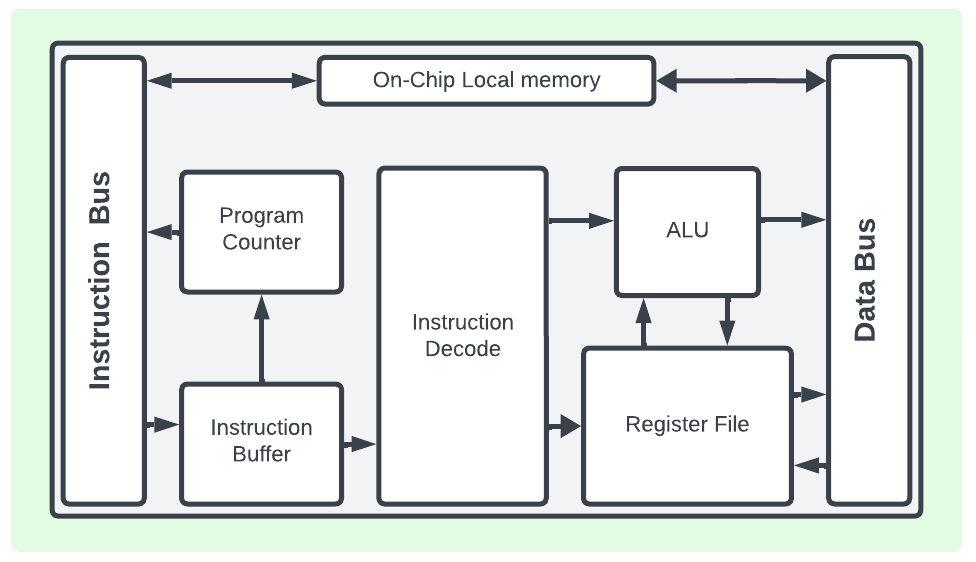
\includegraphics[width=\linewidth]{Images/Microblaze.png}
\caption[Generic Soft Processor Architecture]{Generic Soft Processor Architecture on Programmable Logic. }
\label{fig:AlgoChar}
\end{figure}
%--------------------------------------------------------


\subsubsection{FPGA:}
FPGAs have been utilised for image processing in order to leverage their unique architectural characteristics, such as parallelism, reconfigurability, and low latency. These features enable FPGAs to excel in tasks that demand real-time analysis of image data and require lower power consumption\cite{TakTsuMar08}. 

One major drawback of using FPGAs for image processing is the need to primarily use fixed-point arithmetic. While FPGAs can handle floating-point arithmetic, it often demands too many resources, especially for parallel processing. Vision research typically relies on floating-point algorithms, and adapting them to fixed-point requires a detailed analysis to determine necessary precision at each stage and to work within the FPGA's resource limits\cite{Mac05}. When compared directly to ASIC devices, disregarding cost and design timelines, FPGA implementations are generally less efficient due to the configuration circuitry overhead, which includes I/O and the required SRAM cells to store the current design. This results in larger device sizes and higher power consumption. ASIC design processes also enable circuitry optimisation for faster clock speeds than those achievable on FPGAs\cite{BauDanRoss07}.

\subsubsection{CPU-FPGA:}
Historically, these two components operated independently, each catering to its own application domains. However, in recent years, manufacturers have recognised the complementary strengths of CPUs and FPGAs. This has led to the development of integrated systems, which can be split into two categories, which are soft or hard processors. A soft processor is realised using the programmable logic resources of an FPGA. It's essentially a processor described in a hardware description language, such as VHDL or Verilog, which is then synthesised and mapped onto the FPGA's logic blocks. This design offers flexibility, allowing designers to modify the architecture, add custom instructions, or adjust interfaces as needed, with Xilinx MicroBlaze\cite{AMD_2023} and Intel Nios V\cite{Intel_2023} being notable examples. In contrast, a hard processor is a physical processor core embedded directly into the FPGA silicon which is optimised and hard-wired for better performance and efficiency. The ARM Cortex cores found in newer Xilinx's Zynq FPGAs\cite{AMDSoftProcess} are typically connected to the programmable logic elements through an AXI (Advanced eXtensible Interface) protocol for efficient data transfer and communication. 

Initially, soft CPUs were utilised for pre-processing, task scheduling, and resource management. However, collaborative execution, where tasks are computed by both accelerators, have emerged as a prominent approach for increasing application performance, as demonstrated in the literature \cite{HuaChEL19, RajDarSum23, YiaRos05}. In image processing, soft processors have been shown to be more energy efficient and have comparable runtimes than their counterpart discrete processors for low-high complexity algorithms, which is shown in the works \cite{SidAmmin19,CheCha10,HonOlePol14}. The performance gains extend into the deep learning domain such as CNNs are presented in literature \cite{MelCapDeri28,ZhaPra17,zenpras20,MossNurSim17}.

In summary, hard processors typically outperform soft processors in both speed and resource utilisation due to their independence from FPGA fabric speed and separate chip placement, resulting in enhanced clock speeds and efficient data path designs. Soft processors excel in power efficiency and adaptability, catering to scenarios prioritising energy-conscious designs and dynamic modifications during rapid prototyping and development stages. The architectural distinctions align each processor type with specific application requirements within FPGA-based computing landscapes.


\subsection{CPU-GPU-FPGA Architectures}
\begin{table}[t]
\centering
\setlength{\extrarowheight}{0pt}
\addtolength{\extrarowheight}{\aboverulesep}
\addtolength{\extrarowheight}{\belowrulesep}
\setlength{\aboverulesep}{0pt}
\setlength{\belowrulesep}{0pt}
\caption{Energy and Runtime Speedup of CPU-GPU-FPGA heterogeneous architecture implementations compared to single GPU. The Table only includes works where algorithms are partitioned and processed on all accelerators.}
\label{CPUGPUFPGA}
\resizebox{\linewidth}{!}{%
\begin{tabular}{c|c|c|c|c|c|c} 
\toprule
\rowcolor[rgb]{0.753,0.753,0.753} \textbf{Work} & \multicolumn{2}{c|}{\begin{tabular}[c]{@{}>{\cellcolor[rgb]{0.753,0.753,0.753}}c@{}}\textbf{Heterogeneous}\\\textbf{ Platform}\end{tabular}} & \begin{tabular}[c]{@{}>{\cellcolor[rgb]{0.753,0.753,0.753}}c@{}}\textbf{Partitioning}\\\textbf{ Strategy}\end{tabular} & \textbf{Algorithms} & \begin{tabular}[c]{@{}>{\cellcolor[rgb]{0.753,0.753,0.753}}c@{}}\textbf{Energy }\\\textbf{ Gain}\end{tabular} & \multicolumn{1}{c|}{\begin{tabular}[c]{@{}>{\cellcolor[rgb]{0.753,0.753,0.753}}c@{}}\textbf{Runtime}\\\textbf{ Speedup}\end{tabular}} \\ 
\midrule
\multirow{2}{*}{\begin{tabular}[c]{@{}c@{}}Hyungmin C,\\ etal \cite{ChoLeeLee22}\end{tabular}} & GPU+CPU & ARM+P100 & \multirow{2}{*}{Element-wise} & \multirow{2}{*}{\begin{tabular}[c]{@{}c@{}}Long \\ Short-term\\ Memory\end{tabular}} & \multirow{2}{*}{$\sim$0.34x} & \multirow{2}{*}{$\sim$4.2x} \\ 
\cline{2-3}
 & FPGA & \begin{tabular}[c]{@{}c@{}}Zync\\ Ultrascale\end{tabular} &  &  &  &  \\ 
\midrule
\multirow{3}{*}{\begin{tabular}[c]{@{}c@{}}Hosseinabady M, \\ etal \cite{Hosseinabady2019HeterogeneousFE}\end{tabular}} & GPU+CPU & ARM+Jetson TX1 & \multirow{3}{*}{Element-wise} & Histogram & $\sim$2.29x & $\sim$1.79x \\ 
\cline{2-3}\cline{5-7}
 & \multirow{2}{*}{FPGA} & \multirow{2}{*}{\begin{tabular}[c]{@{}c@{}}Virtex-7\\ Zync\\ Ultrascale\end{tabular}} &  & \begin{tabular}[c]{@{}c@{}}Dense Matrix-Vector\\ Multiplication\end{tabular} & $\sim$1.19x & $\sim$1.48x \\ 
\cline{5-7}
 &  &  &  & \begin{tabular}[c]{@{}c@{}}Sparse Matrix-Vector\\ Multiplication\end{tabular} & $\sim$1.23x & $\sim$1.25x \\ 
\midrule
\multirow{2}{*}{\begin{tabular}[c]{@{}c@{}}Yuexuan T,\\ etal \cite{TuSad19}\end{tabular}} & GPU+CPU & ARM+Jetson TX2 & \multirow{2}{*}{Hybrid} & \multirow{2}{*}{\begin{tabular}[c]{@{}c@{}}LeNet-5\\ N=16\end{tabular}} & \multirow{2}{*}{$\sim$2.11x} & \multirow{2}{*}{$\sim$1.3x} \\ 
\cline{2-3}
 & FPGA & Nexys Artix-7 &  &  &  &  \\ 
\midrule
\multirow{3}{*}{\begin{tabular}[c]{@{}c@{}}Carballo-Hernandez,\\ etal \cite{CarballoHernandez2021WhyIF}\end{tabular}} & GPU+CPU & ARM+Jetson TX2 & \multirow{3}{*}{Layer-Wise} & SqueezeNet Fire & $\sim$1.34x & $\sim$1.01x \\ 
\cline{2-3}\cline{5-7}
 & \multirow{2}{*}{FPGA} & \multirow{2}{*}{\begin{tabular}[c]{@{}c@{}}Cyclone-10 \\ GX\end{tabular}} &  & MobileNet V2 Bottleneck & $\sim$1.55x & $\sim$1.26x \\ 
\cline{5-7}
 &  &  &  & Shufflenet V2 Stage & $\sim$1.39x & $\sim$1.35x \\ 
\midrule
\multirow{3}{*}{\begin{tabular}[c]{@{}c@{}}Sumeet N,\\ etal \cite{SumRaw22}\end{tabular}} & GPU+CPU & ARM+A100 & \multirow{3}{*}{\begin{tabular}[c]{@{}c@{}}Grouped \\Layer-Wise\end{tabular}} & ResNet-18 & $\sim$1.14x & \multirow{3}{*}{-} \\ 
\cline{2-3}\cline{5-6}
 & \multirow{2}{*}{FPGA} & \multirow{2}{*}{\begin{tabular}[c]{@{}c@{}}Xilinx Alveo\\ U280\end{tabular}} &  & ResNet-50 & $\sim$1.08x &  \\ 
\cline{5-6}
 &  &  &  & VGG16-bn & $\sim$1.12x &  \\
\bottomrule
\end{tabular}
}
\end{table}
FPGAs offer the advantage of direct hardware mapping for efficient implementation of CNNs\cite{NguNguKim19}, but they are often constrained by limited on-chip resources\cite{ShawSai19}. The complexity and size of state-of-the-art CNNs often exceed the available logic and memory resources on a single FPGA chip. To mitigate this limitation, a heterogeneous approach can be employed where different layers of the CNN are mapped onto both FPGA and GPU platforms. This leverages the FPGA's efficiency for specific layers while utilising the GPU's computational power for more complex layers, thereby creating a balanced and optimised system.

Recent work into partitioning and executing algorithms onto heterogeneous CPU-GPU-FPGA architectures has been explored in the literature, collected in Table \ref{CPUGPUFPGA}. The platforms category records the combination of accelerators that compose the heterogeneous platform in which the algorithm has been distributed across. The results for energy gain and runtime speedups are derived from comparing the algorithm executed on a single GPU. Partitioning strategy refers to the level of detail at which operations are divided on a heterogeneous platform. In a coarse-grained implementation, entire algorithms or large functional blocks are distributed across different processors within the system. Conversely, a fine-grained implementation maps individual components or layers of an algorithm to specific processors, allowing for more targeted optimisation and resource utilisation.  Across all studies, a range of $1\sim4\times$ speedup and $1\sim2.3\times$ energy improvement is observed from various partitioning techniques. The key areas identified from all works are that the limiting factors for performance are communication latency, resource availability, coarse partitioning strategies and limited optimisations. In all works, CNN algorithms were implemented partially (\eg Convolution Layer Only) or did not pass data to other accelerators, therefore not utilising true heterogeneity.

\section{ASIC Architecture}
ASICs are highly efficient because they are purpose-built and don't require additional support hardware. They integrate all necessary components on a single chip, minimising external dependencies and reducing overall system complexity, making them ideal for streamlined and dedicated image processing tasks\cite{RivPenMolo18, kyrPapEli19}. VPUs have been shown to achieve similar performance to reference CPUs, GPUs and FPGAs. Additionally, benchmarking of NPUs within mobile platforms has shown to be better in runtime than desktop CPUs and comparable to GPUs while consuming less energy\cite{IgnTimKul19}. 



\section{Image Processing Optimisations}

% %--------------------------------------------------------
% \begin{figure}[tb]
% \centering
% 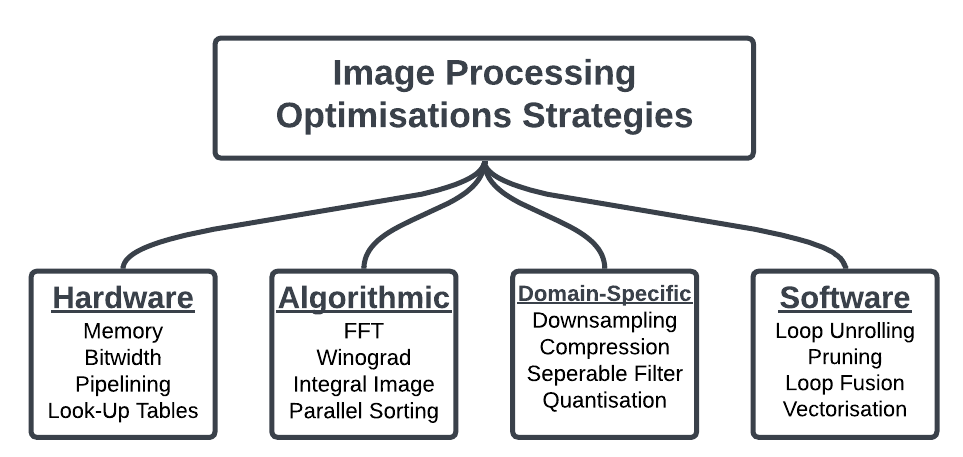
\includegraphics[width=\linewidth]{Images/OptimisationOverview.png}
% \caption{ Popular Image-Processing Optimisations Deployed in Applications}
% \label{fig:OptimisationOverview}
% \end{figure}
% %--------------------------------------------------------


Optimisations are necessary for improving overall system performance, There are three primary categories. First, Hardware optimisations which include optimising memory architectures, computation engine and integrating additional accelerators. Algorithmic optimisations focus on improving the computational procedures, ensuring efficient solving strategies. Lastly, domain-specific optimisations leverage domain knowledge and characteristics inherent to image processing which aim to improve performance, accuracy, and computational efficiency. This section explores optimisation techniques tailored for image processing and CNN algorithms across various hardware accelerators, primarily focused on FPGAs.

\subsection*{Hardware Optimisations}
In image processing, memory usage primarily contributes to overall energy consumption and runtime, especially when algorithms require complete frames to be stored in memory\cite{FanZhanYu17}. However, accelerators such as FPGAs have resource limitations, making efficient utilisation critical for meeting performance, size, and power constraints\cite{HajBenWal18}. Hardware-based memory optimisations can be classified into on-chip and off-chip categories:

\begin{itemize}
    \item On-chip: Involves optimising the use of fast but limited on-chip memory resources like Block RAM in FPGAs or L1/L2 caches in CPUs and GPUs.
    \item Off-chip: focuses on optimising the use of larger but slower off-chip memory like DDR RAM.
\end{itemize}

\textbf{Line buffers} are a memory optimisation technique used in convolution-based algorithms by minimising redundant memory access. The first few lines of the image or signal are loaded into the line buffer, marking the only time these lines are fetched from the main memory. As the convolution operation progresses through the image or signal, the lines already in the buffer are reused to calculate multiple output pixels, thereby eliminating the need to fetch the same lines from the main memory again. When moving to the next set of lines, the buffer shifts, discarding the oldest line and fetching a new one to ensure that the lines immediately needed for the convolution are always available. This data reuse and line shifting minimises the number of times the slower main memory has to be accessed. Line buffers have been explored throughout literature \cite{SonLeeKo14,FanZhaYan17,ZhaXiaHu07,AsaMaeYam09}. Ping-pong buffers employ a dual-buffering scheme, where two or more buffers alternate roles in a synchronised manner. This approach allows one buffer to be filled with new data while the other is being processed, thereby increasing the throughput by speeding up the read/write process \cite{JiaXiaZha14,BaiZhaHua18,liuzoudan19}.

\begin{figure}[tb]
\centering
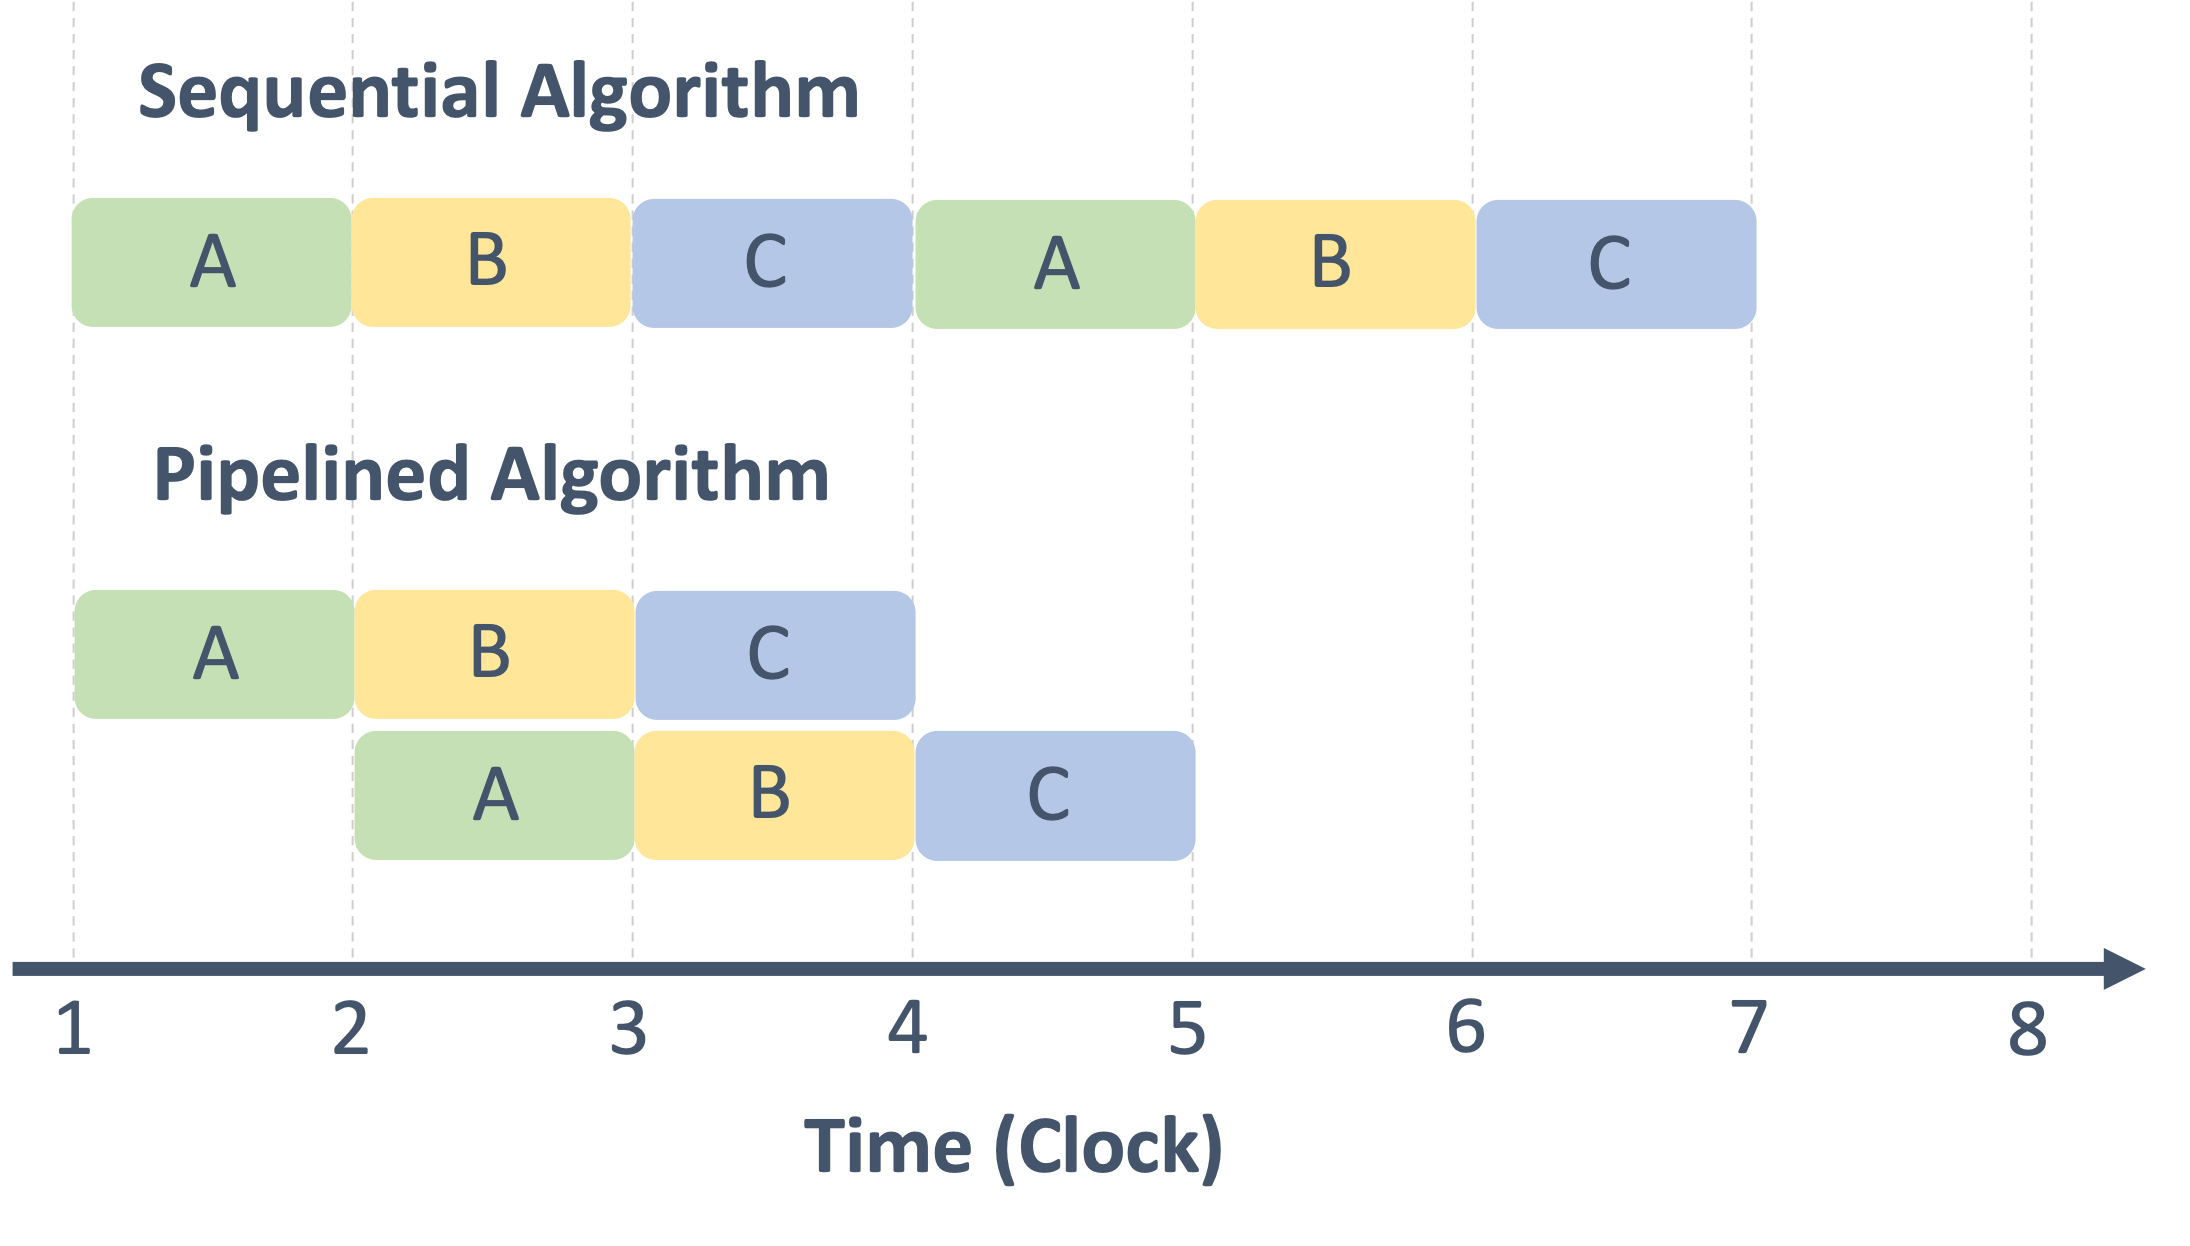
\includegraphics[width=\linewidth]{Images/Pipelining.png}
\caption[Hardware Pipelining Optimisation]{Hardware Pipelining: concurrent processing of multiple stages in a computational task, enhancing throughput and reducing latency.}
\label{fig:pipelining}
\end{figure}

\textbf{Pipelining} is a technique used to increase the throughput by partitioning complex operations into discrete, independent stages implemented within logic elements like LUTs and flip-flops. Each stage performs a specific operation and is clocked separately, allowing for concurrent execution of multiple data elements across stages shown in \Fig{pipelining}. In the works of, Jiang~\etal\cite{JiaXiaZha14} and Bai~\etal\cite{BaiZhaHua18}, significantly improved throughput in their designs, the data generated by each operation was transferred to the next operation without storage, reducing resource consumption and off-chip latency. Additionally, It is important to ensure stage independence for maximum parallelism and to balance resource utilisation to avoid bottlenecks.

\textbf{Look-up tables} (LUTs) are an effective optimisation technique to increase efficiency\cite{RyuNisTos09,MesvAI01}. LUTs pre-compute and store the results of frequently used operations, allowing for rapid retrieval and eliminating the need for redundant calculations. In addition, for more complex expressions, such as square roots or multiplying and dividing by an arbitrary number, look-up tables (LUT) and raster based incremental methods can offer improved performance.

\textbf{Memory architecture }can significantly impact both performance and energy efficiency, especially when dividing on-chip memory into smaller blocks to allow parallel access and reduce latency. However, the choice of parallelism influences the required memory organisation and, consequently, the total energy consumption, which is explored in literature\cite{KadLakDav16,KadLak15}. Following on previous works, Tessier~\etal\cite{TessBetzNet07} showed on-chip power reduction through converting user-defined memory specifications to on-chip FPGA memory block resources. FPGAs often have fixed-size memory that may not align well with the task at hand, leading to energy overhead. Partitioning techniques are therefore required to efficiently manage the storage and processing needs of image data. In the work, Garcia~\etal\cite{GarBhoSte19}, showed that effectively partitioning image frames into BRAMs in order to maximise utilisation (ie, minimise the number of required on-chip memories) can reduce power consumption without affecting the performance. Various off-chip caching systems have been developed to mitigate the latency overheads, such as a three-level memory access architecture proposed by Zhang~\etal\cite{ZhaWeiChe19}. This architecture includes off-chip memory, on-chip buffers, and local memories. Nonetheless, the system entails significant waiting times for valid signals between Block RAMs (BRAMs) and off-chip memory, introducing delays.


\textbf{Approximate computing }techniques can significantly improve computational throughput and energy efficiency in image processing tasks when implemented on FPGAs\cite{Mit16}. These methods trade off a small degree of accuracy for performance gains. Two primary strategies are generally used: the first leverages approximate arithmetic for reduced-precision calculations, while the second aims to decrease the total number of operations without substantially affecting output quality. These approaches can be integrated into the learning or optimisation stages to balance both accuracy and computational demands effectively. One study has shown using lower-bit precision like INT8 and INT4 significantly speeds up neural network inference on various architectures. For example, INT8 inference led to up to 5.02× speedup on GPUs, and INT4 added another 50-60\% speed gain. Mix-precision further improved ResNet50's speed by 2\% without accuracy loss. These benefits extend to non-GPU platforms, achieving up to 2.35× speedup \cite{AmiSehzhe21}. 


\subsubsection*{CNN Hardware Optimisations}
CNNs have now become a popular method of feature extraction and classification. Therefore, this section explores hardware-based optimisation techniques that improve performance. Optimising CNNs on hardware accelerators requires careful algorithm-to-hardware mapping and resource management. The convolutional and fully connected layers are typically the most resource-intensive in terms of both computational logic and memory footprint. Specifically, the storage of high-precision weights and biases for these layers can consume substantial portions of on-chip memory, while the multiply accumulate (MAC) operations required for convolutions and activation's demand significant computational resources as discussed by Laith~\etal\cite{LaiJinAmj21}.


Multiple techniques address these challenges. Firstly, pruning is a compression technique that reduces the model's complexity\cite{Ree93}. These methods identify and remove weights and neurons that contribute minimally to the model's predictive performance, usually based on certain statistical or empirical thresholds. Pruning lessens the memory footprint, reducing the storage required for high-precision weights and biases. At its simplest level, pruning removes the smallest weights, setting them to zero as demonstrated by Song~\etal\cite{han2016deep}. When optimised for energy consumption, pruning techniques that target the least energy-consuming weights achieved a $1.74\times$ gain in efficiency compared to traditional approaches \cite{yang2017designing}. In both methods, the pruned network is fine-tuned to maintain the classification accuracy. Multiple studies demonstrate that pruning eliminates $53\%$ to $85\%$ of weights in a CNNs convolutional and fully connected layers while losing around $0.5\sim1\%$ accuracy \cite{NIPS2015_ae0eb3ee,HeZhaSun17}. Table \ref{tab:hardware_optimisations} summarises optimisations techniques found in hardware.

\begin{table}
\centering
\setlength{\extrarowheight}{0pt}
\addtolength{\extrarowheight}{\aboverulesep}
\addtolength{\extrarowheight}{\belowrulesep}
\setlength{\aboverulesep}{0pt}
\setlength{\belowrulesep}{0pt}
\caption{Summary of Hardware Optimisation Techniques}
\label{tab:hardware_optimisations}
\resizebox{\linewidth}{!}{%
\begin{tabular}{c|l} 
\toprule
\rowcolor[rgb]{0.753,0.753,0.753} \textbf{Optimisation Technique} & \multicolumn{1}{c}{\textbf{Description}}                                                                          \\ 
\midrule
Pipelining                                                        & Concurrent processing of tasks in stages within a pipeline.                                                       \\ 
\midrule
Vectorisation                                                     & Performing operations on entire vectors of data in a single instruction.                                          \\ 
\midrule
Cache Optimisation                                                & Enhancing data locality and minimising cache misses for improved memory access.                                   \\ 
\midrule
Line Buffer                                                       & Storing and processing a line of data at a time; optimising access patterns and reducing memory bandwidth usage.  \\ 
\midrule
Look-Up Table                                                     & Using precomputed values stored in a table for quick retrieval; enhancing computational efficiency.               \\ 
\midrule
\begin{tabular}[c]{@{}c@{}}Memory \\Architecture\end{tabular}     & Optimising the design and organisation of memory systems for efficient data access.                               \\ 
\midrule
\begin{tabular}[c]{@{}c@{}}Approximate \\Computing\end{tabular}   & Allowing imprecise calculations without prioritising accuracy.                                                    \\
\bottomrule
\end{tabular}
}
\end{table}




\subsection*{Domain-Specific Optimisations}
Domain-specific optimisations within the imaging domain are methods tailored to increase the performance of applications. These optimisations leverage the unique characteristics of image processing. Such optimisations often involve exploiting properties like spatial locality, symmetry, and redundancy present in images. In literature, there has been very little research on platform agnostic domain-specific optimisations of imaging algorithms on FPGAs.  Domain-specific tools and optimisations, particularly in areas such as compilers~\cite{RaagBarCon13,TanChoRez11,ChrMehUdayBon21}, have been explored but not yet reached maturity.

In the field of image processing, domain-specific optimisations aim to significantly reduce computational load while maintaining consistent accuracy. Examples of such optimisations include down-sampling~\cite{LinDon06}, approximation\cite{SharZha16}, data-type conversion~\cite{YonLiGuo01}, kernel size adjustments~\cite{NikMaiLon17}, bit-width modification~\cite{WanLouQui18}, and the complete removal of certain operations. Although hardware acceleration techniques for algorithms on CPUs, GPUs, and FPGAs have been extensively researched~\cite{WanWenYan15,SteFraStu14,RisBlaWan13}, these studies generally focus only on target algorithms. In contrast, there has been limited work on exploring the performance and accuracy trade-offs of domain-specific optimisations of imaging algorithms specifically for FPGAs.


\textbf{Downsampling} is a popular method used to reduce the amount of data in an image by selectively removing samples. This involves reducing the resolution of an image by eliminating pixels, usually through averaging or taking the value of a representative pixel in a local neighbourhood. The aim is to decrease computational complexity and storage requirements, making it easier to process and analyse the data. However, downsampling comes with the trade-off of losing some level of detail, which may be critical for certain applications. It is essential to choose an appropriate downsampling factor and method to balance computational efficiency with the preservation of important features in the data.


\textbf{Fast Fourier Transform} is an algorithm to compute the Discrete Fourier Transform (DFT) and its inverse in a more efficient manner. It capitalises on the properties of symmetry and periodicity in the Fourier domain to reduce the number of arithmetic operations. Instead of directly convolving spatial or time-domain signals, FFT first transforms both the input signal and the kernel into the frequency domain. Here, the convolution operation transforms into a simpler element-wise multiplication. After this multiplication, an inverse FFT (IFFT) is applied to bring the data back to the spatial or time domain. The FFT algorithm reduces the computational complexity from \(O(n^2)\) for direct convolution to \(O(n \log n)\), making it highly efficient, especially for larger kernels. The use of FFTs in image processing is found in many works \cite{RioDuh92,FiaCad06,ZhaCheSon16}. However, FFT is hardware-intensive due to its high memory bandwidth requirements and arithmetic complexity, which can lead to increased power consumption.

Additional work by Qiao~\etal~\cite{QiaReiOli19} proposed a minimum cut technique to search fusible kernels recursively to improve data locality. Rawat \etal~\cite{RawPraVad} proposed multiple tiling strategies that improved shared memory and register resources. However, such papers propose constrained domain-specific optimisation strategies that exclusively target CPU and GPU hardware. In related work, Reiche~\etal~\cite{ReiKonMar15} proposed domain knowledge to optimise image processing accelerators using high-level abstraction tools such as domain-specific languages (DSL) and reusable IP-cores. Additional optimisation techniques commonly used in general-purpose computing, such as loop unrolling, fission, and fusion, do not map effectively onto FPGA architectures due to the distinct operational paradigms and resource constraints inherent to FPGA design. Consequently, there is a need for the development of accelerator-agnostic and domain-specific optimisation strategies that can be universally applied across diverse computational platforms, including CPUs, GPUs, and FPGAs, for a more cohesive and efficient heterogeneous design.



\subsection*{Algorithmic Optimisations}
Algorithmic optimisations refer to techniques employed to exploit mathematical properties or patterns in the data being processed. Strategies may include the use of more efficient data structures, dynamic programming, divide and conquer techniques, and algorithmic transformations. Convolution operations are used in many image processing algorithms which typically account for the majority of computation time. Various algorithmic convolution optimisation strategies are discussed below:

\begin{itemize}
    \item The \textit{Strassen}\cite{STRASSEN1969} algorithm optimises matrix multiplication through recursive partitioning. Given two \(n \times n\) matrices, \(A\) and \(B\), it divides each into four submatrices and recursively computes seven intermediate products (\(M_1\) to \(M_7\)). These products are combined to yield the final matrix using additions and subtractions. The algorithm's time complexity of \(O(n^{\log_2{7}})\) improves upon the \(O(n^3)\) complexity of naive multiplication, particularly advantageous for larger matrices. However, its practicality diminishes for smaller matrices due to increased constant factors and memory requirements associated with additional operations. The algorithm has shown to be effective in reducing the computational complexity without losing accuracy in CNN algorithms\cite{ZhaWanWan18}. 

    \item The \textit{Winograd}\cite{winograd1980arithmetic} filter algorithm utilises minimal filtering algorithms to perform convolutions, particularly advantageous for small kernel sizes \( K \leq 3 \). It transforms the convolution operation into a set of polynomial multiplications in a transformed domain. The idea is to decompose the convolution into smaller, overlapping tiles and then apply the Winograd transformation to each tile separately. This results in a significant reduction in the number of multiplicative operations, which are computationally more expensive than additive operations. Numerous works in literature implementing and comparing Winograd performance \cite{Lavin2015FastAF, YepKo20}. In comparison to FFT-based methods which also reduce the number of multiplications by transforming the convolution into a point-wise multiplication in the frequency domain. However, these methods introduce the overhead of complex-to-real transformations and are more computationally intensive for small kernel sizes due to the increased number of additions and the need for padding.
\end{itemize}

% In the domain of CNNs, algorithmic optimisations have been used to decrease runtime of convolutional and fully connected (FC) layers, computational transformations can be applied to feature maps and kernels. The aim is to vectorise the computations and minimise the number of arithmetic operations required during inference. Convolutional layers and fully connected layers in CNNs are commonly implemented using General Matrix Multiply \texttt{GEMM} method\cite{KimNamJun17,CheDiJai16}. In the FC layer of neural networks, \texttt{GEMM} is particularly effective for batch processing feature maps (FMs). These FMs are organised into a \( CHW \times B \) matrix, where \( C \) represents the number of channels, \( H \) for height, \( W \) for width, and \( B \) for the batch size. This structuring allows weights to be loaded just once for each batch, thereby optimising computational throughput and memory bandwidth. This method is valuable since the bulk of weights in CNNs are found in FC layers. Utilising \texttt{GEMM} boosts computational speed and becomes more efficient as the sparsity of the FC weight matrix increases, making it a useful optimisation technique in FC layers.

Specific image processing algorithms often require sorting pixels (e.g., median filtering). These algorithms can benefit from parallel sorting network algorithm optimisations. Sorting networks consist of a predefined sequence of compare-and-swap operations, often organised in a pipeline or tree-like structure, enabling simultaneous execution. In the case of median filtering, sorting networks such as Batcher's Odd-Even Mergesort\cite{Bat68} can be implemented to sort the values in the input window in parallel, thereby reducing time complexity\cite{KimKimSun15}. 

In CNNs, algorithmic optimisations are commonly used to reduce runtime for both convolutional and fully connected (FC) layers. General Matrix Multiply (\texttt{GEMM}) is a key method for implementing these layers, as indicated in \cite{KimNamJun17,CheDiJai16}. In the FC layer, \texttt{GEMM} proves effective for batch processing feature maps (FMs), organised as a \( CHW \times B \) matrix. In which \( C \) represents the number of channels, \( H \) for height, \( W \) for width, and \( B \) for the batch size. This approach optimises computational throughput and memory bandwidth by loading weights just once per batch. Given that FC layers house the majority of CNN weights, \texttt{GEMM} significantly enhances computational speed, especially with increasing sparsity in the FC weight matrix. 




\section{High-Level Synthesis}
\begin{table}
\centering
\caption{Commercial \& Academic High-Level Synthesis Compilers.}
\label{tab:HLS}
\resizebox{\linewidth}{!}{%
\begin{tabular}{c|c|c|c|c|c} 
\hline
\rowcolor[rgb]{0.753,0.753,0.753} \textbf{Compiler} & \textbf{Owner} & \textbf{Year} & \textbf{License} & \textbf{Input} & \multicolumn{1}{c}{\textbf{Output}} \\ 
\hline
Vitis \cite{Vitis} & Xilinx & 2013 & Commercial & C++ & VHDL/Verilog \\ 
\hline
HDL Coder  \cite{mathworks} & Mathworks & 2019 & Commercial & Matlab/Simulink & VHDL/Verilog \\ 
\hline
Intel HLS \cite{intelHLS} & Intel & 2017 & Commercial & C++ & VHDL/Verilog \\ 
\hline
Hardcaml \cite{janestreet} & Jane Street & 2018 & Open Source & Ocaml & VHDL/Verilog \\ 
\hline
Stratus HLS \cite{cadence} & Candence & 2015 & Commercial & C/C++/SystemC & RTL \\ 
\hline
AUGH  \cite{augh} & TIMA Lab. & 2012 & Academia & C subset & VHDL \\ 
\hline
Shang \cite{Shang} & U. Illinois & 2013 & Academia & C subset & Verilog \\
\hline
\end{tabular}
}
\end{table}

High-level synthesis (HLS) is a potential solution to increase the productivity of real-time image processing development on FPGAs. In order to close the performance gap between the manual and HLS-based FPGA designs, various code optimisations that exploit FPGA architecture for potential speedups are made available in today’s HLS tools.  At present, there are various high-level synthesis compilers that are being developed commercially and in academia, shown in table \ref{tab:HLS}.


Efficient code optimisation by HLS compilers is vital in real-time image processing applications, where the goal is to minimise execution time and resource utilisation \cite{SolJinSen19}. Furthermore, the quality of generated Register Transfer Level (RTL) descriptions in High-Level Synthesis (HLS) is found to be influenced by the high-level language used, prompting a need for optimised approaches \cite{ConLiuPra12}. Notably, comparative research underscores significant performance gaps between HLS-based designs and manually crafted counterparts for intricate applications \cite{JasMuhYi11,RupLiaLi11,LiaRupLi12}. Noteworthy disparities of up to 40 times in performance have been documented, particularly evident in demanding tasks like high-definition stereo matching.

Several contemporary avenues in HLS compiler optimisation merit exploration. In the work \cite{HuaLiaCan13}, investigates the impact of compiler optimisations on hardware generated by HLS tools, highlighting the significance of both the optimisation strategies and their sequential application order in enhancing the RTL output quality. In addition, a subsequent study \cite{ChaYanBen17}, refines the understanding of HLS-based real-time image processing design optimisations. Applying a sequence of optimisation techniques, this approach showcases comparable performance when benchmarked against alternative methodologies and industry-standard HLS tools. The optimisations applied in both works include:

\begin{itemize}
    \item \textbf{Function In-lining:} Incorporating functions directly into the code to eliminate function call overhead and improve overall performance.
    
    \item \textbf{Loop Manipulation:} Adjusting loop structures to enhance computational efficiency and reduce processing time.
    
    \item \textbf{Symbolic Expression Manipulation:} Utilising symbolic expressions to manipulate mathematical representations for improved computational speed and precision.
    
    \item \textbf{Loop Unrolling:} Expanding loops by replicating their bodies to reduce loop-control overhead and maximise parallelism.

    \item \textbf{Array Transformation:} Applying various techniques to optimise arrays, the two commonly applied techniques are listed:
        \begin{itemize}
            \item \textbf{Array Partitioning:} Dividing arrays into smaller, more manageable partitions to enhance data locality and optimise parallel processing.
            \item \textbf{Array Reshaping:} Modifying the shape of arrays to better align with computation requirements, improving overall efficiency in data processing.
        \end{itemize}
        
\end{itemize}
 
The advantages of HLS tools observed by Wakabayashi~\etal\cite{Kaz04}, on elevating abstraction levels highlight how expressing designs in higher-level languages like C and C++ can significantly reduce code complexity, making them better at managing complex designs more effectively.



\subsection*{Domain-Specific Languages (DSL)}
% Domain-specific languages (DSLs) raise the level of abstraction by tailoring their focus to particular domains, such as image processing or neural networks. These tools are optimised for their designated domains, potentially delivering higher performance or efficiency for the specific tasks associated with those domains.


\begin{table}[H]
\centering
\caption{Image Processing Targeted Domain-Specific Languages}
\label{tab:DSL}
\resizebox{\linewidth}{!}{%
\begin{tabular}{c|c|c|c|c|c} 
\toprule
\rowcolor[rgb]{0.753,0.753,0.753} \textbf{Compiler} & \textbf{Owner} & \textbf{Year} & \textbf{License} & \textbf{Frontend} & \textbf{Backend} \\ 
\midrule
Halide-Genesis \cite{IshFukMar19} & Akari, Ishikawa Et al. & 2019 & Academia & Actor/Dataflow & VHDL/Verilog \\ 
\midrule
RIPL \cite{SteDunMic18} & Robert,Stewart Et al. & 2018 & Academia & Actor/Dataflow & C/Verilog \\ 
\midrule
HiPacc\cite{MemReiHan16} & R., Membarth Et al. & 2015 & Academia & C++ & VHDL/Verilog \\ 
\midrule
CAPH \cite{SerBerAhm11} & J. Sérot Er al. & 2013 & Academia & Actor/Dataflow & VHDL/SystemC \\ 
\midrule
RVC-CAL \cite{JanMatRau10} & EFPL & 2010 & Academia & Actor/Dataflow & C/Verilog \\
\bottomrule
\end{tabular}
}
\end{table}


A domain-specific language (DSL) is a specialised programming language for a particular domain, such as image processing.  The following paragraphs look into some recent developments of DSLs within image processing. In contrast to C/C++ with HLS tools, DSLs provide clearer syntax, rigorous semantic checks and possible compiler domain optimisations for improved generated code. A summary of available DSLs is found in Table \ref{tab:DSL}.


Richard, Membarth \etal \cite{MemReiHan16} proposed a new DSL and source-to-source compiler for image processing called 'Hipacc'. They show that domain knowledge can be captured to generate tailored implementations for C-based HLS from a common high-level DSL description targeting FPGAs and GPUs. The image processing algorithms that were generated in VHDL/Verilog code from the DSL are evaluated by comparing them with hand-written register transfer level (RTL) implementations. The results show that the HLS still has deficiencies in contrast to the RTL but enables rapid design space exploration. The Hipacc framework does not generate the hardware descriptor language but relies on Xilinx's HLS tools for generated HDL optimisations.

In the work by Jocelyn, Serot \etal \cite{SerBerAhm11} presented CAPH, a DSL suited to implementing stream-processing based applications on FPGA. CAPH relies upon the actor/dataflow model of computation and the tool suite also contains a reference interpreter and a compiler producing both SystemC and VHDL code. CAPH was evaluated by implementing a simple real-time motion detection on an FPGA platform. This was done to validate the overall methodology and to identify key issues. The results established three research directions to improve CAPH. The first is assessing the tools on larger and more complex applications and comparing them with hand-crafted RTL in terms of resource usage and runtime. The second research direction is improving the compiler and optimising the generated VHDL code. Third, applying static analysis techniques to actor behaviours to statically estimate the size of FIFO channels.

%Furthermore, one method to scale the comparison between both versions of RTL is to automatically compare manual implemented RTL code to HLS generated by generating synthesisable code with a auto-tuner to optimise as close to manual RTL.\cite{RasTorAmi23}.

Another DSL for FPGAs was proposed by Robert, Stewart \etal\cite{SteDunMic18} called RIPL. The aim is to increase throughput by maximising clock frequency and minimising resource usage to fit complex algorithms onto FPGAs. RIPL introduces an algorithmic skeleton to express image processing algorithms which are then exploited to generate deep pipelines of highly parallel and memory-efficient image processing components. The data-flow graph generated is expressed in CAL actor language and is compiled into Verilog. The DSL was used to implement image watermarking and multi-dimensional subband decomposition algorithms. 

\section{Benchmarking}
Benchmarking is a relatively established concept in computing, serving as a crucial tool to gauge the performance of various systems. Identifying the most suitable hardware platform becomes imperative, especially when aiming for efficiency and performance. Yet, the challenge lies in determining this without investing significant time and understanding into implementations. Thus, benchmarking measures performance and aids in making informed decisions about hardware compatibility for complex algorithms.

Numerous benchmarking studies have been conducted on a variety of accelerators, including FPGA~\cite{GauAltPin16}, GPU~\cite{AllHorAgar08}, TPU~\cite{JouYouPat18}, and NPU~\cite{qi2023vpuem}. These studies assess performance using specific metrics and facilitate comparisons between different hardware platforms~\cite{QasMurDen19}. Additionally, recent interest in the industry has begun to develop suites such as MLPerf~\cite{RedJanChe2020} and DataPerf~\cite{mazumder2023dataperf} to establish a standardised ML benchmarking and evaluation to allow comparison of inference/training chips or models.


Early work in heterogeneous benchmarking was the introduction of the Rodinia suite in 2009~\cite{CheBoyMic09}. Rodinia comprises applications and kernels that embody the behaviours of the Berkeley dwarfs. These are a taxonomy of 13 computational patterns widely used in various scientific domains. The suite also addresses communication, synchronisation, and power consumption issues. However, Rodinia does not leverage newer features, such as advanced heterogeneous programming constructs, half/mixed precision, tensor computations, and libraries that enhance communication between architectures. Instead, Rodinia focuses on more abstract algorithms rather than micro-benchmarks that target specific components.

Scalable Heterogeneous Computing (SHOC)~\cite{DanMarMcC10} developed in 2010 as another benchmark suite targeting heterogeneous systems. The suite primarily focused on scientific computing workloads, including common kernels such as matrix multiply, fast Fourier transform, and Stencil computation. The benchmark is divided into two testing methods: The stress tests use computationally demanding kernels to identify OpenCL devices with bad memory, insufficient cooling, or other device component problems. The other tests measure many
aspects of system performance on several synthetic kernels as well as common parallel operations and algorithms. SHOC supports various versions of benchmarking, from serial to testing inter-communication between architectures. Every application in the SHOC suite operates within a cohesive framework that allows users to define specific testing parameters, including the desired number of iterations. The framework can also capture intricate metrics, such as floating-point operations per second (FLOPS). The drawback to SHOC is that it focuses on basic parallel algorithms, thus missing the nuance of real-world applications; just like Rodinia, it has not been updated to test modern algorithms and cannot scale to larger problem sizes.

In recent work, Mirovia~\cite{Hu2019MiroviaAB} builds upon both Rodinia and SHOC, designed to leverage the newer evolving architectures. While also representing a diverse set of application domains. This includes a particular focus on deep neural networks. Mirovia aims to characterise modern heterogeneous systems better. The benchmark suite falls short in the range of hardware it can target, being limited to Compute Unified Device Architecture (CUDA) enabled GPU only. Other work focuses on a single domain area; \textit{QuTiBench}~\cite{BloHalLis} is a multi-tiered framework for neural networks which introduces optimisation strategies such as quantisation, which is essential for specific accelerators such as FPGAs. Only the classification stage of the image-signal processing pipeline is tested within the framework; therefore, determining the full performance scope of a vision system is difficult. Reuther~\etal~\cite{ReuAlbMich19} proposed a survey and benchmarked machine learning algorithms on commercial low-power ASICs and a CPU. However, such papers propose benchmarks and frameworks for specific algorithms or target singular architectures, focusing only on execution time performance. In addition, power consumption and memory transfer metrics are often missing in such benchmarks, which is a driving factor for embedded systems with limited energy.


\section{Evaluated Image Processing Algorithms}
This section outlines the implementation details on hardware (primarily FPGA) and the rationale behind the selection of various algorithms evaluated in the subsequent chapters. All algorithms were partly chosen due to their popular use in many image processing pipelines and varying complexity. The CPU and GPU image processing implementations of all algorithms are derived from OpenCV \cite{opencv_library}.  The FPGA implementations have been reviewed in literature to develop widely adopted methods (Algorithmically the same as CPU \& GPU for fair comparison), which, at best, are close to the most optimal design.

\begin{itemize}
    \item \textbf{RGB2Grey, Image Addition, Subtraction:} These operations serve as fundamental building blocks in image processing pipelines. Converting images to grayscale simplifies processing tasks, reduces memory usage, and enhances contrast for improved feature detection. Grayscale images directly represent luminance, making them useful for detecting subtle brightness variations. In addition, grey images have widespread compatibility, require less storage space, and can help reduce noise levels, resulting in clearer images for analysis. Image addition can adjust brightness or contrast by adding or subtracting constant values, while subtraction can isolate foreground objects through background subtraction or detect changes in scenes over time. 

    The FPGA colour conversion module declares parameters for the dimensions of the image (m columns by n rows) and defines registers to store the input colour image in BMP format and the resulting grayscale image. Upon initialisation, the module reads the input colour image data from a BMP file into memory. Then, it iterates over each pixel in the image, extracting the red, green, and blue colour values and calculating their sum. This sum is divided by 3 to obtain the grayscale value, which is stored in a register. The image addition and subtraction module functions by performing pixel-wise arithmetic operations between corresponding pixels in two input images. The modules primarily use registers and combinational logic to perform pixel-wise addition/subtraction of two images. 
    
    \item \textbf{Resizing:} Resizing operations are essential for various image processing applications, including scaling images for different display resolutions or aspect ratios. Many algorithms and CNN architectures require images to be resized to reduce computation complexity.

    The \texttt{imageResize} module facilitates the resizing of input image data by adjusting its width and depth based on specified scaling factors. The resizing operation involves updating counters for tracking column, row, and pixel positions within the image. As the module receives valid input data and a ready signal, it increments these counters accordingly. When the counters reach the desired scaling factors for width and depth, the module resets them to zero, effectively resizing the image. The output image data is synchronized with the clock signal and becomes valid only when both the column and row counters are zero, ensuring proper alignment with the resized image dimensions.
    
    \item \textbf{Erode, Dilate:} Morphological operations like erosion and dilation are commonly used for tasks such as image segmentation and feature extraction. 
     The module \texttt{erodeDilate} operates on grayscale images represented by 8-bit pixel values. A 3x3 buffer array is utilised to store neighbouring pixel values for each input image pixel. Upon initialisation or reset, the buffers and output values are cleared. As new pixel values arrive with each clock cycle, the buffer contents are shifted accordingly. 
    
    For erosion, the module computes the logical AND operation of all pixels in the 3x3 neighbourhood, resulting in the minimum pixel value. Conversely, dilation computes the logical OR operation, resulting in the maximum pixel value. These operations are performed on the buffer contents corresponding to the current pixel position. Finally, the resulting eroded or dilated pixel value is output along with its validity signal.
    
    \item \textbf{Box Filter, Gaussian Filter:} Filters like the box filter and Gaussian filter are fundamental for image smoothing and noise reduction. 

    The Verilog code comprises modules designed for linear filters. The "line Buffer" module functions as a storage mechanism for incoming pixel data, organising it into line buffers to facilitate subsequent convolution operations. It efficiently manages the storage and shifting of pixel data as needed. The "imageControl" module orchestrates the flow of pixel data, determining when to initiate reading and writing operations based on the availability of data and signalling when to begin filtering. It tracks the total number of pixels processed to ensure accurate filtering across the image. The "conv" module is responsible for executing the convolution operation itself. It performs element-wise multiplication of pixel values with corresponding kernel coefficients and aggregates the results to generate the convolved pixel output.
    
    \item \textbf{Sobel Filter, Median Filter:} The Sobel filter is widely used for edge detection, while the median filter is effective for noise removal. The Sobel operator consists of two 3x3 kernels: one for detecting vertical edges and the other for horizontal edges. The module takes nine input pixel values corresponding to the 3x3 neighbourhood surrounding a central pixel. These input pixels are named according to their relative positions: Within the module, two instances of the \texttt{matrix\textunderscore mul} module compute the gradient components along the x-axis (\texttt{gx}) and y-axis (\texttt{gy}) using the Sobel kernels. The result of each multiplication operation is squared to obtain the squared gradient magnitudes in the \texttt{gx\textunderscore squared} and \texttt{gy\textunderscore squared} wires. These squared magnitudes are then added together to compute the overall squared gradient magnitude in the \texttt{squared\textunderscore sum} wire. The \texttt{sqrt} module calculates the square root of the squared gradient magnitude.

    The \texttt{median filter} module takes in pixel values (pixel\textunderscore in) of image width and operates on a square filtering window of fixed size.  Within each processing cycle, the module updates the window with new pixel values, sorts the window values to find the median value, and outputs the median as the filtered pixel value (pixel\textunderscore out). The algorithm maintains internal registers to store the window and the histogram-based sorted window of pixel values. During reset, the internal registers are initialised, and processing flags are reset. 
    
    \item \textbf{White Balance:} White balance adjustment is essential for achieving accurate colour representation in images captured under different lighting conditions. 

    \texttt{WhiteBalance} module is designed to perform white balance adjustment on an input image by adjusting the red, green, and blue colour channels. It takes in pixel values for the red, green, and blue channels of the image.

    The module maintains buffers to accumulate the pixel values for each colour channel (\texttt{red\textunderscore sum}, \texttt{green\textunderscore sum}, \texttt{blue\textunderscore sum}) and a register to count the number of pixels processed (\texttt{pixel\textunderscore count}). These registers store the accumulated sums and count, respectively.
    On each clock cycle, the module accumulates the pixel values and updates the count. Then, it calculates the average pixel values for each colour channel by dividing the accumulated sum by the pixel count. Finally, it applies the white balance coefficients to adjust the colour channels accordingly.

    \item \textbf{Linearization: \& Gamma Correction} Linearization and gamma correction are essential in image processing, ensuring consistent pixel representation and adjusting brightness and contrast for good visual images, making them ideal for bench-marking.
    
    The \texttt{Linearization} module is designed to linearize the pixel values of an input image, effectively scaling them to a range between 0 and 1. The module takes an 8-bit pixel value as input and outputs the corresponding linearized value. It employs simple arithmetic logic to divide the input pixel value by 255, the maximum value in an 8-bit system, thereby scaling it to the desired range. The linearization process occurs on each clock cycle, ensuring real-time processing of image data.

    \texttt{GammaCorrection} module applies gamma correction to an input pixel value using a real gamma value of 2.2. The module operates synchronously with the clock signal and includes a reset input for initialisation. Inside the module, it takes the input pixel value and applies a power function with an integer approximation of the gamma value. The function then converts the gamma-corrected integer value back to the [0, 255] range to ensure compatibility with pixel representations. The module continuously applies the gamma correction function to the input pixel value on each clock cycle. The output pixel value is updated accordingly. The input and output pixel values are stored in registers.
    
    \item \textbf{GEMM:} GEMM algorithm serves as a base building block for numerous image processing and deep learning operations  due to their algorithmic efficiency in performing matrix multiplications. The algorithm is computed in many areas of ML, such as fully-connected layers, recurrent layers such as recurrent neural networks, Long short-term memory or Gated recurrent unit, and convolutional layers. Benchmarking GEMM allows for assessing the computational performance and scalability of hardware architectures across a wide range of image processing and deep learning algorithms. The optimised FPGA GEMM implementations used for evaluation are provided by Xilinx\cite{AMDGEMM} library.
    
    \item \textbf{FFT (DFT):} Fast Fourier Transform (FFT) are found in various operations in imaging algorithms by enabling efficient frequency domain analysis and manipulation of images for tasks such as filtering, convolution, registration, texture analysis, edge detection, compression, and super-resolution imaging. Xilinx provided FFT IP-block\cite{AMDFFT} is used in the benchmarking. The module implements the Cooley-Tukey FFT algorithm for computing both forward and inverse DFTs of sample sizes that are powers of 2. 
    
    \item \textbf{STREAM:} Memory bandwidth and latency are important metrics because they directly impact the speed and efficiency of data transfer between the processor and memory. Therefore, when benchmarking image processing algorithms, measuring memory bandwidth and latency provides insights into how efficiently the algorithms utilise memory resources, helping assess their overall performance and scalability. The implementation used for FPGAs are from HPCC \textunderscore FPGA benchmarking suite\cite{hpcc_fpga}.
    
    \item \textbf{Demosaicing:} Demosaicing algorithms are essential for reconstructing colour images from Bayer-pattern sensor data which are common filter used in vision systems. The algorithm is a good choice to benchmark since most vision systems use Bayer filter. Xilinx provided de-mosaicing IP-block\cite{AMDDemosiac} is used in the benchmarking. The demosaicing algorithm used is a bilinear interpolation, where missing colour values in a Bayer-filtered image are estimated by averaging neighbouring pixel values.
    
    \item \textbf{SIFT:} Scale-Invariant Feature Transform (SIFT) is a widely used technique for feature extraction in image processing applications. The FPGA implementation is discussed in Section \ref{SIFTHardwareDesc}.
    
    \item \textbf{CNN (Classification):} Convolutional Neural Networks (CNNs) have become significantly popular methods for image classification, object detection/segmentation tasks. Xilinx Deep Learning Processor Unit (DPU) is used to implement both optimised ResNet-18 and MobilnetV2 architectures\cite{AMDDPU}.
\end{itemize}


\section{Conclusion}
This chapter delves into the discussion and evaluation of diverse heterogeneous architecture implementations, tools, and optimisation strategies. The literature review emphasises that specific processing architectures, such as GPUs, FPGAs, and VPUs, exhibit greater efficiency in executing imaging algorithms than CPUs, owing to their architectural properties (\eg SIMD, DSP Slice) and depending on algorithmic features like parallelisation and data dependencies. Moreover, these architectures to exploit their advantages leads to further performance gains. Various optimisations have also been shown to enhance the efficiency of image processing algorithms, encompassing techniques such as algorithm replacement, hardware (memory management) and pipelining schemes. However, the knowledge gap is evident in the lack of a systematic approach or set of strategies for partitioning imaging algorithms onto the appropriate hardware accelerators in a heterogeneous platform, nor a comprehensive rationale for such decisions. In addition, there are no end-to-end implementations of CNN and feature extraction algorithms utilising CPU-GPU-FPGA architectures. The absence of image-domain-guided optimisations and understanding of trade-offs further complicates achieving optimal performance and efficiency. Hence, within the scope of this thesis, a robust benchmarking framework that guides algorithm partitioning along with domain-specific optimisation strategies on heterogeneous platforms is proposed.